% Generated by Sphinx.
\def\sphinxdocclass{report}
\documentclass[a4paper,11pt,english]{sphinxmanual}
\usepackage[utf8]{inputenc}
\DeclareUnicodeCharacter{00A0}{\nobreakspace}
\usepackage{cmap}
\usepackage[T1]{fontenc}
\usepackage{babel}
\usepackage{times}
\usepackage[Bjarne]{fncychap}
\usepackage{longtable}
\usepackage{sphinx}
\usepackage{multirow}
\setcounter{tocdepth}{2}

\title{Introduction to the Linux Commandline for NGS Analyses}
\date{September 18, 2013}
\release{1.1}
\author{Grainne Kerr, Holger Dinkel, Jon Fuller, Matt Betts}
\newcommand{\sphinxlogo}{
\includegraphics{HUBLogo.png}\par}
\renewcommand{\releasename}{}
\makeindex

\makeatletter
\def\PYG@reset{\let\PYG@it=\relax \let\PYG@bf=\relax%
    \let\PYG@ul=\relax \let\PYG@tc=\relax%
    \let\PYG@bc=\relax \let\PYG@ff=\relax}
\def\PYG@tok#1{\csname PYG@tok@#1\endcsname}
\def\PYG@toks#1+{\ifx\relax#1\empty\else%
    \PYG@tok{#1}\expandafter\PYG@toks\fi}
\def\PYG@do#1{\PYG@bc{\PYG@tc{\PYG@ul{%
    \PYG@it{\PYG@bf{\PYG@ff{#1}}}}}}}
\def\PYG#1#2{\PYG@reset\PYG@toks#1+\relax+\PYG@do{#2}}

\expandafter\def\csname PYG@tok@gd\endcsname{\def\PYG@tc##1{\textcolor[rgb]{0.63,0.00,0.00}{##1}}}
\expandafter\def\csname PYG@tok@gu\endcsname{\let\PYG@bf=\textbf\def\PYG@tc##1{\textcolor[rgb]{0.50,0.00,0.50}{##1}}}
\expandafter\def\csname PYG@tok@gt\endcsname{\def\PYG@tc##1{\textcolor[rgb]{0.00,0.27,0.87}{##1}}}
\expandafter\def\csname PYG@tok@gs\endcsname{\let\PYG@bf=\textbf}
\expandafter\def\csname PYG@tok@gr\endcsname{\def\PYG@tc##1{\textcolor[rgb]{1.00,0.00,0.00}{##1}}}
\expandafter\def\csname PYG@tok@cm\endcsname{\let\PYG@it=\textit\def\PYG@tc##1{\textcolor[rgb]{0.25,0.50,0.56}{##1}}}
\expandafter\def\csname PYG@tok@vg\endcsname{\def\PYG@tc##1{\textcolor[rgb]{0.73,0.38,0.84}{##1}}}
\expandafter\def\csname PYG@tok@m\endcsname{\def\PYG@tc##1{\textcolor[rgb]{0.13,0.50,0.31}{##1}}}
\expandafter\def\csname PYG@tok@mh\endcsname{\def\PYG@tc##1{\textcolor[rgb]{0.13,0.50,0.31}{##1}}}
\expandafter\def\csname PYG@tok@cs\endcsname{\def\PYG@tc##1{\textcolor[rgb]{0.25,0.50,0.56}{##1}}\def\PYG@bc##1{\setlength{\fboxsep}{0pt}\colorbox[rgb]{1.00,0.94,0.94}{\strut ##1}}}
\expandafter\def\csname PYG@tok@ge\endcsname{\let\PYG@it=\textit}
\expandafter\def\csname PYG@tok@vc\endcsname{\def\PYG@tc##1{\textcolor[rgb]{0.73,0.38,0.84}{##1}}}
\expandafter\def\csname PYG@tok@il\endcsname{\def\PYG@tc##1{\textcolor[rgb]{0.13,0.50,0.31}{##1}}}
\expandafter\def\csname PYG@tok@go\endcsname{\def\PYG@tc##1{\textcolor[rgb]{0.20,0.20,0.20}{##1}}}
\expandafter\def\csname PYG@tok@cp\endcsname{\def\PYG@tc##1{\textcolor[rgb]{0.00,0.44,0.13}{##1}}}
\expandafter\def\csname PYG@tok@gi\endcsname{\def\PYG@tc##1{\textcolor[rgb]{0.00,0.63,0.00}{##1}}}
\expandafter\def\csname PYG@tok@gh\endcsname{\let\PYG@bf=\textbf\def\PYG@tc##1{\textcolor[rgb]{0.00,0.00,0.50}{##1}}}
\expandafter\def\csname PYG@tok@ni\endcsname{\let\PYG@bf=\textbf\def\PYG@tc##1{\textcolor[rgb]{0.84,0.33,0.22}{##1}}}
\expandafter\def\csname PYG@tok@nl\endcsname{\let\PYG@bf=\textbf\def\PYG@tc##1{\textcolor[rgb]{0.00,0.13,0.44}{##1}}}
\expandafter\def\csname PYG@tok@nn\endcsname{\let\PYG@bf=\textbf\def\PYG@tc##1{\textcolor[rgb]{0.05,0.52,0.71}{##1}}}
\expandafter\def\csname PYG@tok@no\endcsname{\def\PYG@tc##1{\textcolor[rgb]{0.38,0.68,0.84}{##1}}}
\expandafter\def\csname PYG@tok@na\endcsname{\def\PYG@tc##1{\textcolor[rgb]{0.25,0.44,0.63}{##1}}}
\expandafter\def\csname PYG@tok@nb\endcsname{\def\PYG@tc##1{\textcolor[rgb]{0.00,0.44,0.13}{##1}}}
\expandafter\def\csname PYG@tok@nc\endcsname{\let\PYG@bf=\textbf\def\PYG@tc##1{\textcolor[rgb]{0.05,0.52,0.71}{##1}}}
\expandafter\def\csname PYG@tok@nd\endcsname{\let\PYG@bf=\textbf\def\PYG@tc##1{\textcolor[rgb]{0.33,0.33,0.33}{##1}}}
\expandafter\def\csname PYG@tok@ne\endcsname{\def\PYG@tc##1{\textcolor[rgb]{0.00,0.44,0.13}{##1}}}
\expandafter\def\csname PYG@tok@nf\endcsname{\def\PYG@tc##1{\textcolor[rgb]{0.02,0.16,0.49}{##1}}}
\expandafter\def\csname PYG@tok@si\endcsname{\let\PYG@it=\textit\def\PYG@tc##1{\textcolor[rgb]{0.44,0.63,0.82}{##1}}}
\expandafter\def\csname PYG@tok@s2\endcsname{\def\PYG@tc##1{\textcolor[rgb]{0.25,0.44,0.63}{##1}}}
\expandafter\def\csname PYG@tok@vi\endcsname{\def\PYG@tc##1{\textcolor[rgb]{0.73,0.38,0.84}{##1}}}
\expandafter\def\csname PYG@tok@nt\endcsname{\let\PYG@bf=\textbf\def\PYG@tc##1{\textcolor[rgb]{0.02,0.16,0.45}{##1}}}
\expandafter\def\csname PYG@tok@nv\endcsname{\def\PYG@tc##1{\textcolor[rgb]{0.73,0.38,0.84}{##1}}}
\expandafter\def\csname PYG@tok@s1\endcsname{\def\PYG@tc##1{\textcolor[rgb]{0.25,0.44,0.63}{##1}}}
\expandafter\def\csname PYG@tok@gp\endcsname{\let\PYG@bf=\textbf\def\PYG@tc##1{\textcolor[rgb]{0.78,0.36,0.04}{##1}}}
\expandafter\def\csname PYG@tok@sh\endcsname{\def\PYG@tc##1{\textcolor[rgb]{0.25,0.44,0.63}{##1}}}
\expandafter\def\csname PYG@tok@ow\endcsname{\let\PYG@bf=\textbf\def\PYG@tc##1{\textcolor[rgb]{0.00,0.44,0.13}{##1}}}
\expandafter\def\csname PYG@tok@sx\endcsname{\def\PYG@tc##1{\textcolor[rgb]{0.78,0.36,0.04}{##1}}}
\expandafter\def\csname PYG@tok@bp\endcsname{\def\PYG@tc##1{\textcolor[rgb]{0.00,0.44,0.13}{##1}}}
\expandafter\def\csname PYG@tok@c1\endcsname{\let\PYG@it=\textit\def\PYG@tc##1{\textcolor[rgb]{0.25,0.50,0.56}{##1}}}
\expandafter\def\csname PYG@tok@kc\endcsname{\let\PYG@bf=\textbf\def\PYG@tc##1{\textcolor[rgb]{0.00,0.44,0.13}{##1}}}
\expandafter\def\csname PYG@tok@c\endcsname{\let\PYG@it=\textit\def\PYG@tc##1{\textcolor[rgb]{0.25,0.50,0.56}{##1}}}
\expandafter\def\csname PYG@tok@mf\endcsname{\def\PYG@tc##1{\textcolor[rgb]{0.13,0.50,0.31}{##1}}}
\expandafter\def\csname PYG@tok@err\endcsname{\def\PYG@bc##1{\setlength{\fboxsep}{0pt}\fcolorbox[rgb]{1.00,0.00,0.00}{1,1,1}{\strut ##1}}}
\expandafter\def\csname PYG@tok@kd\endcsname{\let\PYG@bf=\textbf\def\PYG@tc##1{\textcolor[rgb]{0.00,0.44,0.13}{##1}}}
\expandafter\def\csname PYG@tok@ss\endcsname{\def\PYG@tc##1{\textcolor[rgb]{0.32,0.47,0.09}{##1}}}
\expandafter\def\csname PYG@tok@sr\endcsname{\def\PYG@tc##1{\textcolor[rgb]{0.14,0.33,0.53}{##1}}}
\expandafter\def\csname PYG@tok@mo\endcsname{\def\PYG@tc##1{\textcolor[rgb]{0.13,0.50,0.31}{##1}}}
\expandafter\def\csname PYG@tok@mi\endcsname{\def\PYG@tc##1{\textcolor[rgb]{0.13,0.50,0.31}{##1}}}
\expandafter\def\csname PYG@tok@kn\endcsname{\let\PYG@bf=\textbf\def\PYG@tc##1{\textcolor[rgb]{0.00,0.44,0.13}{##1}}}
\expandafter\def\csname PYG@tok@o\endcsname{\def\PYG@tc##1{\textcolor[rgb]{0.40,0.40,0.40}{##1}}}
\expandafter\def\csname PYG@tok@kr\endcsname{\let\PYG@bf=\textbf\def\PYG@tc##1{\textcolor[rgb]{0.00,0.44,0.13}{##1}}}
\expandafter\def\csname PYG@tok@s\endcsname{\def\PYG@tc##1{\textcolor[rgb]{0.25,0.44,0.63}{##1}}}
\expandafter\def\csname PYG@tok@kp\endcsname{\def\PYG@tc##1{\textcolor[rgb]{0.00,0.44,0.13}{##1}}}
\expandafter\def\csname PYG@tok@w\endcsname{\def\PYG@tc##1{\textcolor[rgb]{0.73,0.73,0.73}{##1}}}
\expandafter\def\csname PYG@tok@kt\endcsname{\def\PYG@tc##1{\textcolor[rgb]{0.56,0.13,0.00}{##1}}}
\expandafter\def\csname PYG@tok@sc\endcsname{\def\PYG@tc##1{\textcolor[rgb]{0.25,0.44,0.63}{##1}}}
\expandafter\def\csname PYG@tok@sb\endcsname{\def\PYG@tc##1{\textcolor[rgb]{0.25,0.44,0.63}{##1}}}
\expandafter\def\csname PYG@tok@k\endcsname{\let\PYG@bf=\textbf\def\PYG@tc##1{\textcolor[rgb]{0.00,0.44,0.13}{##1}}}
\expandafter\def\csname PYG@tok@se\endcsname{\let\PYG@bf=\textbf\def\PYG@tc##1{\textcolor[rgb]{0.25,0.44,0.63}{##1}}}
\expandafter\def\csname PYG@tok@sd\endcsname{\let\PYG@it=\textit\def\PYG@tc##1{\textcolor[rgb]{0.25,0.44,0.63}{##1}}}

\def\PYGZbs{\char`\\}
\def\PYGZus{\char`\_}
\def\PYGZob{\char`\{}
\def\PYGZcb{\char`\}}
\def\PYGZca{\char`\^}
\def\PYGZam{\char`\&}
\def\PYGZlt{\char`\<}
\def\PYGZgt{\char`\>}
\def\PYGZsh{\char`\#}
\def\PYGZpc{\char`\%}
\def\PYGZdl{\char`\$}
\def\PYGZhy{\char`\-}
\def\PYGZsq{\char`\'}
\def\PYGZdq{\char`\"}
\def\PYGZti{\char`\~}
% for compatibility with earlier versions
\def\PYGZat{@}
\def\PYGZlb{[}
\def\PYGZrb{]}
\makeatother

\begin{document}

\maketitle
\tableofcontents
\phantomsection\label{index::doc}



\chapter{Introduction to the Linux Commandline}
\label{introduction:introduction-to-the-linux-commandline}\label{introduction:introduction-to-the-linux-commandline-for-ngs-analyses}\label{introduction::doc}

\section{Why Use the Commandline}
\label{introduction:why-use-the-commandline}\begin{itemize}
\item {} 
It's \textbf{fast}. Productivity is a word that gets tossed around a lot by so-called power users, but the command line can really streamline your computer use, assuming you learn to use it right.

\item {} 
It's \textbf{easier to get help}. The command line may not be the easiest thing to use, but it makes life a whole lot easier for people trying to help you and for yourself when looking for help, especially over the internet. Many times it's as simple as the helper posting a few commands and some instructions and the recipient copying and pasting those commands. Anyone who has spent hours listening to someone from tech support say something like, “OK, now click this, then this, then select this menu command” knows how frustrating the GUI alternative can be.

\item {} 
It's nearly \textbf{universal}. There are hundreds of Linux distros out there, each with a slightly different graphical environment. Thankfully, the various distros do have one common element: the command line. There are distro-specific commands, but the bulk of commands will work on any Linux system.

\item {} 
It's \textbf{powerful}. The companies behind those other operating systems try their best to stop a user from accidentally screwing up their computer. Doing this involves hiding a lot of the components and tools that could harm a computer away from novices. Linux is more of an open book, which is due in part to its prominent use of the command line.

\end{itemize}


\section{General Remarks Regarding Using UNIX/Linux Systems}
\label{introduction:general-remarks-regarding-using-unix-linux-systems}\begin{itemize}
\item {} 
\textbf{Test before run}. Anything written here has to be taken with a grain of salt. On another system – be it a different Linux distribution or another UNIXoid operating system – you might find the same command but without the support of some of the options tought here. It is even possible, that the same option has a different meaning on another system. With this in mind always make sure to test your commands (especially the “dangerous” ones which remove or modify files) when switching from one system to the other.

\item {} 
\textbf{The Linux/UNIX environment}. The behaviour of many commands is influenced or controlled by the so-called “environment”. This environment is the sum of all your environment variables. Some of these environment variables will be shown towards the end of this course.

\item {} 
\textbf{UPPERCASE, lowercase}. Don’t forget that everything is case-sensitive.

\item {} 
\textbf{The Filesystem}. Linux filesystems start on top at the root directory (sic!) “/” which hierarchically broadens towards the ground.  The separator between directories or directories and files in Linux is the slash (“/”).

\end{itemize}
\begin{figure}[htbp]
\centering
\capstart

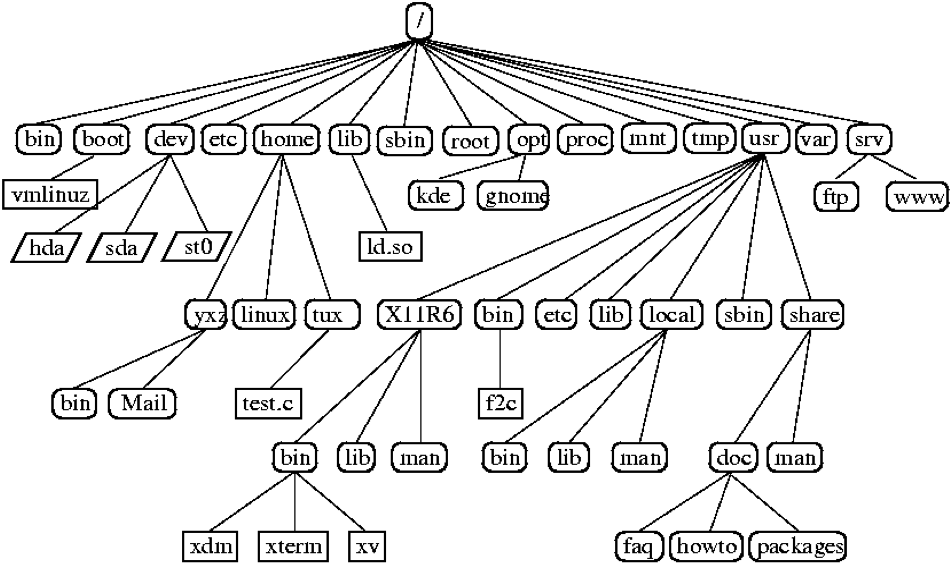
\includegraphics{filesystem.png}
\caption{Depending on the Linux distribution you might or might not find all of above
directories. Most important directories for you are \code{/bin} and \code{/usr/bin}
(sometimes also \code{/usr/local/bin}) which contain the user software, \code{/home} which
usually contains the users’ homedirectories and \code{/tmp} which can be used to store
temporary data (beware: Its content is regularly removed!).}\label{introduction:figure-filesystem}\end{figure}

\begin{notice}{note}{Note:}
The terms “directory” and “folder” are used interchangeably in this document.
\end{notice}


\section{General Structure of Linux Commands}
\label{introduction:general-structure-of-linux-commands}
Many linux commands have options and accept arguments. Options are a set of switch-like parameters
while arguments are usually free text input (such as a filename).
\begin{figure}[htbp]
\centering
\capstart

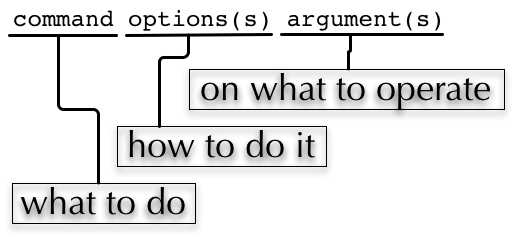
\includegraphics{LinuxCommandStructure.png}
\caption{General structure of Linux commands.}\end{figure}

Commandline options (sometimes called comandline switches) commonly have one of the two following
forms: The short form \code{-s} (just a single character) or the long form \code{-{-}string.} E.g.
\begin{quote}

\begin{Verbatim}[commandchars=\\\{\}]
\PYGZgt{} man \PYGZhy{}h
\PYGZgt{} man \PYGZhy{}\PYGZhy{}help
\end{Verbatim}
\end{quote}

Short options are usually – though not always – concatenable:
\begin{quote}

\begin{Verbatim}[commandchars=\\\{\}]
\PYGZgt{} ls \PYGZhy{}l \PYGZhy{}A \PYGZhy{}h
\PYGZgt{} ls \PYGZhy{}lAh
\end{Verbatim}
\end{quote}

Some options require an additional argument, which is added with a blank to the short form and with an equal sign to the long form:
\begin{quote}

\begin{Verbatim}[commandchars=\\\{\}]
\PYGZgt{} ls \PYGZhy{}I “*.pdf”
\PYGZgt{} ls \PYGZhy{}\PYGZhy{}ignore\PYG{o}{=}”*.pdf”
\end{Verbatim}
\end{quote}

Since Linux incorporates commands from different sources, options can be available in one or both forms and you’ll also encounter options with no dash at all and all kinds of mixtures:
\begin{quote}

\begin{Verbatim}[commandchars=\\\{\}]
\PYGZgt{} tar cf file.tar \PYGZhy{}C .. file/
\PYGZgt{} ps auxgww
\end{Verbatim}
\end{quote}


\section{A Journey Through the Commands}
\label{introduction:a-journey-through-the-commands}
Please note that all examples and usage instructions below are just a glimpse of what you can do and reflect our opinion on what’s important and what’s not. Most of these commands support many more options and different usages. Consult the manpages to find them.
Typographical conventions: Commands and examples are written in Courier.  User Input is written in Courier bold and placeholders are generally written in italic.


\subsection{Getting Help}
\label{introduction:getting-help}\label{introduction:help}
\code{-h/-{-}help} option, no parameters

Many commands support a “help” option, either through \code{-h} or through \code{-{-}help}.
Other commands will show a help page or at least a short usage overview if you provide incorrect commandline options


\subsubsection{man - show the manual page of a command}
\label{introduction:man-show-the-manual-page-of-a-command}
\textbf{Usage}:
\code{man command or file}
\begin{quote}

\begin{Verbatim}[commandchars=\\\{\}]
\PYGZgt{} man man
man\PYG{o}{(}1\PYG{o}{)}

NAME
 man \PYGZhy{} format and display the on\PYGZhy{}line manual pages

SYNOPSIS
 man \PYG{o}{[}\PYGZhy{}acdfFhkKtwW\PYG{o}{]} \PYG{o}{[}\PYGZhy{}\PYGZhy{}path\PYG{o}{]} \PYG{o}{[}\PYGZhy{}m system\PYG{o}{]} \PYG{o}{[}\PYGZhy{}p string\PYG{o}{]} \PYG{o}{[}\PYGZhy{}C config\PYGZus{}file\PYG{o}{]}
\PYG{o}{[}...\PYG{o}{]}
\end{Verbatim}
\end{quote}

For the navigation within a \index{man}man-page see the chapter regarding less below.

\begin{notice}{note}{Note:}
The behaviour of man is dependent of the \$PAGER environment variable
\end{notice}


\paragraph{apropos – list manpages containing a keyword in their description}
\label{introduction:apropos-list-manpages-containing-a-keyword-in-their-description}
\textbf{Usage}: \code{apropos keyword}
\begin{quote}

\begin{Verbatim}[commandchars=\\\{\}]
\PYGZgt{} apropos who
\PYG{o}{[}...\PYG{o}{]}
\PYGZgt{} who                  \PYG{o}{(}1\PYG{o}{)}  \PYGZhy{} show who is logged on
\PYGZgt{} who                  \PYG{o}{(}1\PYG{o}{)}  \PYGZhy{} display who is on the system
\PYGZgt{} whoami               \PYG{o}{(}1\PYG{o}{)}  \PYGZhy{} print effective userid
\end{Verbatim}
\end{quote}

Use \index{apropos}apropos to find candidates for specific tasks


\paragraph{/usr/share/doc}
\label{introduction:usr-share-doc}
The \code{/usr/share/doc} directory in some Linux distributions contains additional documentation of installed software packages


\subsection{Who am I, where am I}
\label{introduction:who-am-i-where-am-i}

\subsubsection{whoami – Print your username}
\label{introduction:whoami-print-your-username}
\textbf{Usage}: \code{whoami}
\begin{quote}

\begin{Verbatim}[commandchars=\\\{\}]
\PYGZgt{} whoami
bg\PYGZus{}36student
\end{Verbatim}
\end{quote}


\subsubsection{hostname – Print the name of the computer}
\label{introduction:hostname-print-the-name-of-the-computer}
\textbf{Usage}: \code{hostname}
\begin{quote}

\begin{Verbatim}[commandchars=\\\{\}]
\PYGZgt{} hostname
pc\PYGZhy{}teach01
\end{Verbatim}
\end{quote}


\subsubsection{pwd – Print the current working directory}
\label{introduction:pwd-print-the-current-working-directory}
\textbf{Usage}: \code{pwd}
\begin{quote}

\begin{Verbatim}[commandchars=\\\{\}]
\PYGZgt{} \PYG{n+nb}{pwd}
/home/bg\PYGZus{}36student
\end{Verbatim}
\end{quote}


\subsubsection{date – Print current date and time}
\label{introduction:date-print-current-date-and-time}
\textbf{Usage}: \code{date}
\begin{quote}

\begin{Verbatim}[commandchars=\\\{\}]
\PYGZgt{} date
Tue Sep 25 19:57:50 CEST 2012
\end{Verbatim}
\end{quote}

\begin{notice}{note}{Note:}
The command \emph{time} does something completely different than \index{date}date and is not used to show the current time.
\end{notice}


\subsection{Moving Around}
\label{introduction:moving-around}

\subsubsection{cd – Change the working directory}
\label{introduction:cd-change-the-working-directory}
\textbf{Usage}: \code{cd {[}new\_directory{]}}
\begin{quote}

\begin{Verbatim}[commandchars=\\\{\}]
\PYG{c}{\PYGZsh{} pwd}
/home/bg\PYGZus{}36student
\PYG{c}{\PYGZsh{} cd /usr/bin}
\PYG{c}{\PYGZsh{} pwd}
/usr/bin
\end{Verbatim}
\end{quote}

Special directories:
\begin{itemize}
\item {} 
“\code{.}”:  The current working directory

\item {} 
“\code{..}”: The parent directory of the current working directory

\item {} 
“\code{\textasciitilde{}}”:  Your homedirectory

\end{itemize}

\begin{notice}{note}{Note:}
Using \index{cd}cd without a directory is equivalent to “\code{cd \textasciitilde{}}” and changes into the users’s homedirectory
\end{notice}

\begin{notice}{note}{Note:}
Please note the difference between absolute paths (starting with ``\code{/}'') and relative paths (starting with a directory name)
\end{notice}

\begin{Verbatim}[commandchars=\\\{\}]
\PYG{n+nv}{\PYGZdl{} }\PYG{n+nb}{pwd}
/usr
\PYG{n+nv}{\PYGZdl{} }\PYG{n+nb}{cd} /bin
\PYG{n+nv}{\PYGZdl{} }\PYG{n+nb}{pwd}
/bin
\end{Verbatim}

\begin{Verbatim}[commandchars=\\\{\}]
\PYGZgt{} \PYG{n+nb}{pwd}
/usr
\PYGZgt{} \PYG{n+nb}{cd }bin
\PYGZgt{} \PYG{n+nb}{pwd}
/usr/bin
\end{Verbatim}


\subsection{See What’s Around}
\label{introduction:see-whats-around}

\subsubsection{ls - List directory contents}
\label{introduction:ls-list-directory-contents}\begin{description}
\item[{\textbf{Usage}:}] \leavevmode
\code{ls {[}options{]} {[}file(s) or directory/ies{]}}

\end{description}

\begin{Verbatim}[commandchars=\\\{\}]
\PYGZgt{} ls
/home/bg\PYGZus{}36student
\PYGZgt{} ls –l /bin/date
\PYGZhy{}rwxr\PYGZhy{}xr\PYGZhy{}x 1 root root 54920 Dec 18  2012 /bin/date
\end{Verbatim}

Useful options:
\begin{optionlist}{3cm}
\item [-l]  
Long listing with permissions, user, group and last modification date
\item [-1]  
Print listing in one column only
\item [-a]  
Show all files (hidden, “.” and “..”)
\item [-A]  
Show almost all files (hidden, but not “.” and “..”)
\item [-F]  
Show filetypes (nothing = regular file, “/” = directory, “*” = executable file, “@” = symbolic link)
\item [-d]  
Show directory information instead of  directory content
\item [-t]  
Sort listing by modification time (most recent on top)
\end{optionlist}


\bigskip\hrule{}\bigskip

\begin{figure}[htbp]
\centering

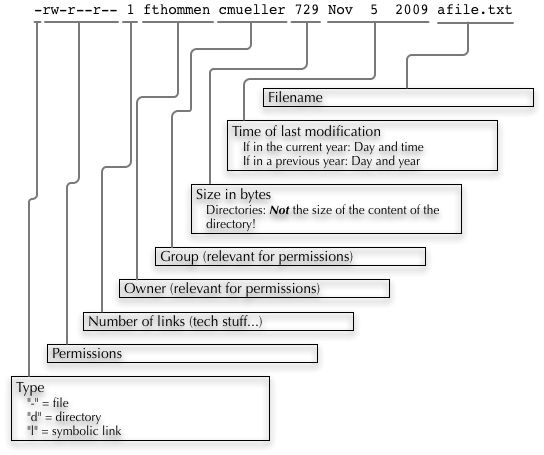
\includegraphics{LongListingDeconstructed.png}
\end{figure}


\bigskip\hrule{}\bigskip



\subsubsection{Digression: Shell globs}
\label{introduction:digression-shell-globs}
Files and folders can’t only be referred to with their full name, but also with so-called “Shell Globs”, which are a kind of simple pattern to address groups of files and folders.  Instead of explicit names you can use the following placeholders:
\begin{itemize}
\item {} 
\code{?:}  Any single character

\item {} 
\code{*:}  Any number of any character (including no character at all)

\item {} 
\code{{[}...{]}:}    One of the characters included in the brackets.  Use “-“ to define ranges  of characters

\end{itemize}

Examples:
\begin{itemize}
\item {} 
\code{*.pdf:}  All files having the extension “.pdf”

\item {} 
\code{?.jpg:}  Jpeg file consisting of only one character

\item {} 
\code{{[}0-9{]}*.txt:} All files starting with a number and having the extension “.txt”

\item {} 
\code{*.???:}  All files having a three-character extension

\end{itemize}

\begin{notice}{note}{Note:}
The special directory “\code{\textasciitilde{}}” mentioned above is a shell glob, too.
\end{notice}


\subsection{Organize Files and Folders}
\label{introduction:organize-files-and-folders}

\subsubsection{touch – Create a file or change last modification date of an existing file}
\label{introduction:touch-create-a-file-or-change-last-modification-date-of-an-existing-file}
\textbf{Usage}:  \code{touch file(s) or directory/ies}
\begin{quote}

\begin{Verbatim}[commandchars=\\\{\}]
\PYGZgt{} ls afile
ls: afile: No such file or directory
\PYGZgt{} touch afile
\PYGZgt{} ls afile
afile
\end{Verbatim}

\begin{Verbatim}[commandchars=\\\{\}]
\PYGZgt{} ls –l \PYGZti{}/exercises/P12931.txt
\PYGZhy{}rw\PYGZhy{}r\PYGZhy{}\PYGZhy{}r\PYGZhy{}\PYGZhy{} 1 dinkel gibson  53K Aug 11 14:21 P12931.txt
\PYGZgt{} touch \PYGZti{}/exercises/P12931.txt
\PYGZgt{} ls –l \PYGZti{}/exercises/P12931.txt
\PYGZhy{}rw\PYGZhy{}r\PYGZhy{}\PYGZhy{}r\PYGZhy{}\PYGZhy{} 1 dinkel gibson  53K Sep 18 19:16 P12931.txt
\end{Verbatim}
\end{quote}


\subsubsection{rm – Remove files and directories}
\label{introduction:rm-remove-files-and-directories}
\textbf{Usage}:  \code{rm {[}options{]} file(s)}
\begin{quote}

\begin{Verbatim}[commandchars=\\\{\}]
rm –r \PYG{o}{[}options\PYG{o}{]} directory/ies
\PYGZgt{} ls afile
afile
\PYGZgt{} rm afile
\PYGZgt{} ls afile
ls: afile: No such file or directory
\end{Verbatim}
\end{quote}

\textbf{Useful options}:
\begin{optionlist}{3cm}
\item [-i]  
Ask for confirmation of each removal
\item [-r]  
Remove recursively
\item [-f]  
Force the removal (no questions, no errors if a file doesn't exist)
\end{optionlist}

\begin{notice}{note}{Note:}
rm without the –i option will usually not ask you if you really want to remove the file or directory
\end{notice}


\subsubsection{mv – Move and rename files and folders}
\label{introduction:mv-move-and-rename-files-and-folders}
\textbf{Usage}:  \code{mv {[}options{]} sourcefile destinationfile}
\begin{quote}

\begin{Verbatim}[commandchars=\\\{\}]
mv \PYG{o}{[}options\PYG{o}{]} sourcefile\PYG{o}{(}s\PYG{o}{)} destinationdirectory
\PYGZgt{} ls *.txt
a.txt
\PYGZgt{} mv a.txt b.txt
\PYGZgt{} ls *.txt
b.txt
\end{Verbatim}
\end{quote}

\textbf{Useful options}:
\begin{optionlist}{3cm}
\item [-i]  
Ask for confirmation of each removal
\end{optionlist}

\begin{notice}{note}{Note:}
You cannot overwrite an existing directory by another one with mv
\end{notice}


\subsubsection{mkdir – Create a new directory}
\label{introduction:mkdir-create-a-new-directory}\label{introduction:mkdir}
\textbf{Usage}:  \code{mkdir {[}options{]} directory}
\begin{quote}

\begin{Verbatim}[commandchars=\\\{\}]
\PYGZgt{} ls adir/
ls: adir/: No such file or directory
\PYGZgt{} mkdir adir
\PYGZgt{} ls adir
\end{Verbatim}
\end{quote}

\textbf{Useful options}:
\begin{optionlist}{3cm}
\item [-p]  
Create parent directories (when creating nested directories)
\end{optionlist}

\begin{Verbatim}[commandchars=\\\{\}]
\textgreater{} mkdir adir/bdir
mkdir: cannot create directory {}`adir/bdir': No such file or directory
\textgreater{} mkdir –p adir/bdir
\end{Verbatim}


\subsubsection{rmdir – Remove an empty directory}
\label{introduction:rmdir-remove-an-empty-directory}
\textbf{Usage}:  \code{rmdir directory}
\begin{quote}

\begin{Verbatim}[commandchars=\\\{\}]
\PYGZgt{} rmdir adir/
\end{Verbatim}
\end{quote}

\begin{notice}{note}{Note:}
If the directory is not empty, rmdir will complain and not remove it
\end{notice}


\subsubsection{cp – Copy files and folders}
\label{introduction:cp-copy-files-and-folders}
\textbf{Usage}:  \code{cp {[}options{]} sourcefile destinationfile}
\begin{quote}

\begin{Verbatim}[commandchars=\\\{\}]
\PYGZgt{} cp P12931.fasta backup\PYGZus{}of\PYGZus{}P12931.fasta
\end{Verbatim}
\end{quote}

\textbf{Useful options}:
\begin{optionlist}{3cm}
\item [-r]  
Copy recursively
\item [-i]  
Interactive operation, ask before overwriting an existing file
\item [-p]  
Preserve owner, permissions and timestamp
\end{optionlist}


\subsection{View Files}
\label{introduction:view-files}

\subsubsection{cat – Print files on terminal (concatenate)}
\label{introduction:cat-print-files-on-terminal-concatenate}
\textbf{Usage}:  \code{cat {[}options{]} file(s)}
\begin{quote}

\begin{Verbatim}[commandchars=\\\{\}]
\PYGZgt{} cat  P12931.fasta backup\PYGZus{}of\PYGZus{}P12931.fasta
\PYG{o}{[}...\PYG{o}{]}
\end{Verbatim}
\end{quote}

\begin{notice}{note}{Note:}
\index{cat}cat only makes sense for short files or for e.g. combining several files into one.  See the redirection examples later
\end{notice}


\subsubsection{less – View and navigate files}
\label{introduction:less-view-and-navigate-files}
\textbf{Usage}:  \code{less {[}options{]} file(s)}
\begin{quote}

\begin{Verbatim}[commandchars=\\\{\}]
\PYGZgt{} less  P12931.fasta backup\PYGZus{}of\PYGZus{}P12931.fasta
\PYG{o}{[}...\PYG{o}{]}
\end{Verbatim}
\end{quote}

\begin{notice}{note}{Note:}
This is the default “pager” for manpages under Linux unless you redefine your \$PAGER environment variable
\end{notice}

\textbf{Navigation within less}:

\begin{tabulary}{\linewidth}{|L|L|}
\hline
\textsf{\relax 
Key(s):
} & \textsf{\relax 
Effect:
}\\
\hline
up, down, right, left:
 & 
use cursor keys
\\

top of document:
 & 
g
\\

bottom of document:
 & 
G
\\

search:
 & 
“/” + search-term
\\

find next match:
 & 
n
\\

find previous match:
 & 
N
\\

quit:
 & 
q
\\
\hline\end{tabulary}



\subsection{Extracting Informations from Files}
\label{introduction:extracting-informations-from-files}

\subsubsection{grep – Find lines matching a pattern in textfiles}
\label{introduction:grep-find-lines-matching-a-pattern-in-textfiles}
\index{grep}Grep is a command-line utility for searching plain-text data sets for lines matching a regular expression.

\textbf{Usage}:  \code{grep {[}options{]} pattern file(s)}
\begin{quote}

\begin{Verbatim}[commandchars=\\\{\}]
\PYGZgt{} grep \PYGZhy{}i ensembl P04637.txt
DR   Ensembl; ENST00000269305; ENSP00000269305; ENSG00000141510.
DR   Ensembl; ENST00000359597; ENSP00000352610; ENSG00000141510.
DR   Ensembl; ENST00000419024; ENSP00000402130; ENSG00000141510.
DR   Ensembl; ENST00000420246; ENSP00000391127; ENSG00000141510.
DR   Ensembl; ENST00000445888; ENSP00000391478; ENSG00000141510.
DR   Ensembl; ENST00000455263; ENSP00000398846; ENSG00000141510.
\end{Verbatim}
\end{quote}

\textbf{Useful options}:
\begin{optionlist}{3cm}
\item [-v]  
Print lines that do not match
\item [-i]  
Search case-insensitive
\item [-l]  
List files with matching lines, not the lines itself
\item [-L]  
List files without matches
\item [-c]  
Print count of matching lines for each file
\end{optionlist}


\subsubsection{head – Print first lines of a textfile}
\label{introduction:head-print-first-lines-of-a-textfile}
\index{head}Head is a program on Unix and Unix-like systems used to display the beginning of a text file or piped data.

\textbf{Usage}:  \code{head {[}options{]} file(s)}
\begin{quote}

\begin{Verbatim}[commandchars=\\\{\}]
\PYGZgt{} head /etc/passwd
root:x:0:0:root:/root:/bin/bash
bin:x:1:1:bin:/bin:/sbin/nologin
daemon:x:2:2:daemon:/sbin:/sbin/nologin
adm:x:3:4:adm:/var/adm:/sbin/nologin
lp:x:4:7:lp:/var/spool/lpd:/sbin/nologin
sync:x:5:0:sync:/sbin:/bin/sync
shutdown:x:6:0:shutdown:/sbin:/sbin/shutdown
halt:x:7:0:halt:/sbin:/sbin/halt
mail:x:8:12:mail:/var/spool/mail:/sbin/nologin
news:x:9:13:news:/etc/news:
\end{Verbatim}
\end{quote}

\textbf{Useful options}:
\begin{optionlist}{3cm}
\item [-n num]  
Print num lines (default is 10)
\end{optionlist}


\subsubsection{tail – Print last lines of a textfile}
\label{introduction:tail-print-last-lines-of-a-textfile}
\textbf{Usage}:  \code{tail {[}options{]} file(s)}
\begin{quote}

\begin{Verbatim}[commandchars=\\\{\}]
\PYGZgt{} tail –n 3 /etc/passwd
xfs:x:43:43:X Font Server:/etc/X11/fs:/sbin/nologin
gdm:x:42:42::/var/gdm:/sbin/nologin
sabayon:x:86:86:Sabayon user:/home/sabayon:/sbin/nologin
\end{Verbatim}
\end{quote}

\textbf{Useful options}:
\begin{optionlist}{3cm}
\item [-n num]  
Print num lines (default is 10)
\item [-f]  
``Follow'' a file (print new lines as they are written to the file)
\end{optionlist}


\subsection{Useful Filetools}
\label{introduction:useful-filetools}

\subsubsection{file – determine the filetype}
\label{introduction:file-determine-the-filetype}
\textbf{Usage}:  \code{file {[}options{]} file(s)}
\begin{quote}

\begin{Verbatim}[commandchars=\\\{\}]
\PYGZgt{} file /bin/date
/bin/date: ELF 32\PYGZhy{}bit LSB executable
\PYGZgt{} file /bin
/bin: directory
\PYGZgt{} file SRC\PYGZus{}HUMAN.fasta
SRC\PYGZus{}HUMAN.fasta: ASCII text
\end{Verbatim}
\end{quote}

\begin{notice}{note}{Note:}
The command \index{file}file uses certain tests and some magic to determine the type of a file
\end{notice}


\subsubsection{which – find a (executable) command}
\label{introduction:which-find-a-executable-command}
\textbf{Usage}:  \code{which {[}options{]} command(s)}
\begin{quote}

\begin{Verbatim}[commandchars=\\\{\}]
\PYGZgt{} which date
/bin/date
\PYGZgt{} which eclipse
/usr/bin/eclipse
\PYGZgt{}
\end{Verbatim}
\end{quote}


\subsubsection{find – search/find files in any given directory}
\label{introduction:find-search-find-files-in-any-given-directory}
\textbf{Usage}:  \code{find {[}starting path(es){]} {[}search filter{]}}
\begin{quote}

\begin{Verbatim}[commandchars=\\\{\}]
\PYGZgt{} find /etc
/etc
/etc/printcap
/etc/protocols
/etc/xinetd.d
/etc/xinetd.d/ktalk
\PYG{o}{[}...\PYG{o}{]}
\PYGZgt{}
\end{Verbatim}
\end{quote}

\code{find} \index{find}is a powerful command with lots of possible search filters.  Refer to the manpage for a complete list.

\textbf{Examples}:
\begin{itemize}
\item {} 
Find by name:

\end{itemize}
\begin{quote}

\begin{Verbatim}[commandchars=\\\{\}]
\PYGZgt{} find . \PYGZhy{}name SRC\PYGZus{}HUMAN.fasta
./SRC\PYGZus{}HUMAN.fasta
\end{Verbatim}
\end{quote}
\begin{itemize}
\item {} 
Find by size: (List those entries in the directory /usr/bin that are bigger than 500kBytes)

\end{itemize}
\begin{quote}

\begin{Verbatim}[commandchars=\\\{\}]
\PYGZgt{} find /usr/bin \PYGZhy{}size +500k
/usr/bin/oparchive
/usr/bin/kiconedit
/usr/bin/opjitconv
\PYG{o}{[}...\PYG{o}{]}
\end{Verbatim}
\end{quote}
\begin{itemize}
\item {} 
Find by type (d=directory, f=file, l=link)

\end{itemize}
\begin{quote}

\begin{Verbatim}[commandchars=\\\{\}]
\PYGZgt{} find . \PYGZhy{}type d
.
./adir
\end{Verbatim}
\end{quote}


\subsection{Useful Terminal Tools}
\label{introduction:useful-terminal-tools}

\subsubsection{clear – Clear the “screen”}
\label{introduction:clear-clear-the-screen}
\textbf{Usage}:  \code{clear}
\begin{quote}

\begin{Verbatim}[commandchars=\\\{\}]
\PYGZgt{} clear
\end{Verbatim}
\end{quote}

In case the output of the terminal/screen gets cluttered, you can use \code{clear} to \index{clear}clear the screen...

If this doesn't work, you can use \code{reset} to perform a re-initialization of the terminal:


\subsubsection{reset – Reset your terminal}
\label{introduction:reset-reset-your-terminal}
\textbf{Usage}:  \code{reset {[}options{]}}
\begin{quote}

\begin{Verbatim}[commandchars=\\\{\}]
\PYGZgt{} reset
\end{Verbatim}
\end{quote}


\subsection{Permissions}
\label{introduction:permissions}
using ls -l to view entries of current directory:
\begin{quote}

\begin{Verbatim}[commandchars=\\\{\}]
\PYGZgt{} ls –l
drwxr\PYGZhy{}xr\PYGZhy{}x 2 dinkel gibson 4096 Sep 17 10:46 adir
lrwxrwxrwx 1 dinkel gibson   15 Sep 17 10:45 H1.fasta \PYGZhy{}\PYGZgt{} H2.fasta
\PYGZhy{}rw\PYGZhy{}r\PYGZhy{}\PYGZhy{}r\PYGZhy{}\PYGZhy{} 1 dinkel gibson  643 Sep 17 10:45 H2.fasta
\end{Verbatim}
\end{quote}
\begin{figure}[htbp]
\centering

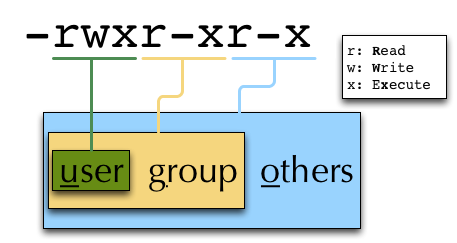
\includegraphics{LinuxPermissions.png}
\end{figure}


\subsubsection{Changing Permissions}
\label{introduction:changing-permissions}
Permissions are set using the \code{chmod} (\index{chmod}change mode ) command.

\textbf{Usage}:  \code{chmod {[}options{]} mode(s) files(s)}
\begin{quote}

\begin{Verbatim}[commandchars=\\\{\}]
\PYGZgt{} ls –l adir
drwxr\PYGZhy{}xr\PYGZhy{}x 2 dinkel gibson 4096 Sep 17 10:46 adir
\PYGZgt{} chmod u\PYGZhy{}w,o\PYG{o}{=}w adir
\PYGZgt{} ls –l adir
dr\PYGZhy{}xr\PYGZhy{}x\PYGZhy{}w\PYGZhy{} 2 dinkel gibson 4096 Sep 17 10:46 adir
\end{Verbatim}
\end{quote}

The mode is composed of

\begin{tabulary}{\linewidth}{|L|L|L|L|L|L|}
\hline
 \multicolumn{2}{|l|}{\textsf{\relax 
Who
}} &  \multicolumn{2}{l|}{\textsf{\relax 
What
}} &  \multicolumn{2}{l|}{\textsf{\relax 
Which permission
}}\\
\hline
u:
 & 
user/owner
 & 
+:
 & 
add this permission
 & 
r:
 & 
read
\\

g:
 & 
group
 & 
-:
 & 
remove this permission
 & 
w:
 & 
write
\\

o:
 & 
other
 & 
=:
 & 
set exactly this permission
 & 
x:
 & 
execute
\\

a:
 & 
all
 &  &  &  & \\
\hline\end{tabulary}


Add executable permission to the group:
\begin{quote}

\begin{Verbatim}[commandchars=\\\{\}]
\PYGZgt{} chmod g+x file
\end{Verbatim}
\end{quote}

Revoke this permission:
\begin{quote}

\begin{Verbatim}[commandchars=\\\{\}]
\PYGZgt{} chmod g\PYGZhy{}x file
\end{Verbatim}
\end{quote}

Allow all to read a directory:
\begin{quote}

\begin{Verbatim}[commandchars=\\\{\}]
\PYGZgt{} chmod a+rx adir/
\end{Verbatim}
\end{quote}


\subsection{Remote access}
\label{introduction:remote-access}
To execute commands at a remote machine/server, you need to log in to this machine. This is done
using the \code{ssh} command (secure shell). In its simplest form, it takes just the machinename as
parameter (assuming the username on the local machine and remote machine are identical):
\begin{quote}

\begin{Verbatim}[commandchars=\\\{\}]
\PYGZgt{} ssh remote\PYGZus{}server
\end{Verbatim}
\end{quote}

\begin{notice}{note}{Note:}
Once logged in, \index{hostname}\index{whoami}use \code{hostname,} \code{whoami,} etc. to
determine on which machine you are currently working and to get a feeling for your
environment!
\end{notice}

To use a different username, you can use either:
\begin{quote}

\begin{Verbatim}[commandchars=\\\{\}]
\PYGZgt{} ssh \PYGZhy{}l username remote\PYGZus{}server
\end{Verbatim}
\end{quote}

or
\begin{quote}

\begin{Verbatim}[commandchars=\\\{\}]
\PYGZgt{} ssh username@remote\PYGZus{}server
\end{Verbatim}
\end{quote}

When connecting to a machine for the first time, it might display a warning:
\begin{quote}

\begin{Verbatim}[commandchars=\\\{\}]
\textgreater{} ssh cln038
The authenticity of host 'cln038 (129.296.243.53)' can't be established.
RSA key fingerprint is 47:a4:0f:7b:c2:0f:ef:91:8e:65:fc:3c:f7:0c:53:8d.
Are you sure you want to continue connecting (yes/no)?
\end{Verbatim}
\end{quote}

Type \emph{yes} here.
If this message appears a second time, you should contact your IT specialist...
\begin{description}
\item[{To \index{exit}\index{disconnect}disconnect from the remote machine, type:}] \leavevmode
\begin{Verbatim}[commandchars=\\\{\}]
\PYGZgt{} \PYG{n+nb}{exit}
\end{Verbatim}

\end{description}

If setup correctly, you can even use \textbf{graphical tools} from the remote server on the local machine.
For this to work, you need to start the ssh session with the \code{-X} parameter:
\begin{quote}

\begin{Verbatim}[commandchars=\\\{\}]
\PYGZgt{} ssh \PYGZhy{}X remote\PYGZus{}server
\end{Verbatim}
\end{quote}

Copying files to and from remote computers can be done using \code{scp}  (secure copy).
The order of parameters is the same as in \code{cp}: first the name of the source, then the name of the destination. Either one can be the remote part.
\begin{quote}

\begin{Verbatim}[commandchars=\\\{\}]
\PYGZgt{} scp localfile server:/remotefile

\PYGZgt{} scp server:/remotefile localfile
\end{Verbatim}
\end{quote}

An alternative username can be provided just as in ssh:
\begin{quote}

\begin{Verbatim}[commandchars=\\\{\}]
\PYGZgt{} scp username@server:/remotefile localfile
\end{Verbatim}
\end{quote}


\subsection{IO and Redirections}
\label{introduction:io-and-redirections}

\subsubsection{Redirect}
\label{introduction:redirect}
\index{redirect}Redirect the output of one program into e.g. a file: (Caution: you can easily overwrite files by this!)
Inserting the current date into a new file:
\begin{quote}

\begin{Verbatim}[commandchars=\\\{\}]
\PYGZgt{} date \PYGZgt{} file\PYGZus{}containing\PYGZus{}date
\end{Verbatim}
\end{quote}

\index{grep}Filtering lines containing the term “src” from FASTA files and inserting them into the file lines\_with\_src.txt:
\begin{quote}

\begin{Verbatim}[commandchars=\\\{\}]
\PYGZgt{} \PYG{n+nb}{cd} \PYGZti{}/exercises/
\PYGZgt{} grep \PYGZhy{}i \PYG{l+s+s2}{\PYGZdq{}src\PYGZdq{}} *.fasta \PYGZgt{} lines\PYGZus{}with\PYGZus{}src.txt
\end{Verbatim}
\end{quote}


\subsubsection{Append}
\label{introduction:append}
\index{append}Append something to a file (rather than overwriting it):
\begin{quote}

\begin{Verbatim}[commandchars=\\\{\}]
\PYGZgt{} date \PYGZgt{}\PYGZgt{} file\PYGZus{}containing\PYGZus{}date
\end{Verbatim}
\end{quote}


\subsubsection{Pipe}
\label{introduction:pipe}\label{introduction:id1}
Use the \index{\textbar{}}\index{pipe}\textbar{} pipe symbol (\code{\textbar{}}) to feed the output of one program into the next program.
Here: use \code{ls} to show the directory contents and then \index{grep}use \code{grep} to only show those that contain fasta in their name:
\begin{quote}

\begin{Verbatim}[commandchars=\\\{\}]
\PYGZgt{} \PYG{n+nb}{cd} \PYGZti{}/exercises
\PYGZgt{} ls \textbar{} grep fasta
EPSINS.fasta
FYN\PYGZus{}HUMAN.fasta
P12931.fasta
SRC\PYGZus{}HUMAN.fasta
\end{Verbatim}
\end{quote}


\subsection{Environment Variables}
\label{introduction:environment-variables}
\index{environment variables}Environment variables are a set of dynamic named values that can affect the way running processes will behave on a computer.


\subsubsection{\$HOME}
\label{introduction:home}
Contains the location of the user's home directory. Although the current user's home directory can also be found out through the
C functions \code{getpwuid} and \code{getuid,} \index{\$HOME}\$HOME is often used for convenience in various shell scripts (and other contexts).

\begin{notice}{note}{Note:}
Do not change this variable unless you have a good reason and you know what you are doing!
\end{notice}


\subsubsection{\$PATH}
\label{introduction:path}\label{introduction:id2}
\index{\$PATH}\$PATH contains a colon-separated list of directories that the shell searches for commands that do not contain a slash in their name
(commands with slashes are interpreted as file names to execute, and the shell attempts to execute the files directly).


\subsubsection{\$PAGER}
\label{introduction:pager}
The \index{\$PAGER}\$PAGER variable contains the path to the program used to list the contents of files through (such \index{less}as \code{less} \index{more}or \code{more}).


\subsubsection{\$PWD}
\label{introduction:pwd}
The \index{\$PWD}\$PWD variable points to the current directory. Equivalent to the output of the command \code{pwd} when called without arguments.


\subsubsection{Displaying environment variables}
\label{introduction:displaying-environment-variables}
\index{environment variables!display}Use \code{echo} to \index{echo}display individual variables \emph{set{}`} \index{env}or \code{env} to view all at once:
\begin{quote}

\begin{Verbatim}[commandchars=\\\{\}]
\PYGZgt{} \PYG{n+nb}{echo} \PYG{n+nv}{\PYGZdl{}HOME}
/localhome/teach01
\PYGZgt{} \PYG{n+nb}{set}
...
\PYGZgt{} env
...
\end{Verbatim}
\end{quote}


\subsubsection{Setting an environment variable}
\label{introduction:setting-an-environment-variable}
Use \code{export} followed by the variable name and the value of the variable (separated by the equal sign) to \index{environment variables!set}\index{set}\index{export}set an environment variable:
\begin{quote}

\begin{Verbatim}[commandchars=\\\{\}]
\PYGZgt{} \PYG{n+nb}{export }\PYG{n+nv}{PAGER}\PYG{o}{=}/usr/bin/less
\end{Verbatim}
\end{quote}

\begin{notice}{note}{Note:}
An environment variable is only valid for your current session. Once you logout of your current session, it is lost or reset.
\end{notice}


\chapter{Exercises}
\label{exercises/exercises_beginner:exercises}\label{exercises/exercises_beginner::doc}

\section{Misc. file tools}
\label{exercises/exercises_beginner:misc-file-tools}\begin{enumerate}
\item {} 
Which tool can be used to determine the type of a file?

\item {} 
Use it on the following files/directories and compare the results:
\begin{enumerate}
\item {} 
\code{/usr/bin/tail}

\item {} 
\code{\textasciitilde{}}

\item {} 
\code{\textasciitilde{}/exercises/SRC\_HUMAN.fasta}

\end{enumerate}

\end{enumerate}


\section{Searching}
\label{exercises/exercises_beginner:searching}\begin{enumerate}
\item {} 
Which tool can be used to search for files or directories?

\item {} 
Use it to find all directories in the \code{\textasciitilde{}/exercises} directory

\item {} 
Search for the file \code{date} in the \code{/bin} directory

\item {} 
List those entries in the directory \code{/bin} that are bigger than 400kBytes

\end{enumerate}


\section{Misc. terminal}
\label{exercises/exercises_beginner:misc-terminal}\begin{enumerate}
\item {} 
Which two tools can be used to redraw/empty the screen?

\end{enumerate}


\section{Permissions}
\label{exercises/exercises_beginner:permissions}\begin{enumerate}
\item {} 
Create a directory called testpermissions (in your homedirectory)

\item {} 
Change your working directory to this new directory

\item {} 
In there, create another directory called adir.

\item {} 
Use the command \code{which date} to find out where the date program is located.

\item {} 
Copy this date program into the directory adir.

\item {} 
Check the permissions of the copied program date

\item {} 
Change the permissions on date to remove the executable permissions.

\item {} 
Check the permissions of the program date

\item {} 
Try running it as \code{./date} or \code{adir/date} (depending on your current working directory)

\item {} 
Change the permissions back so that the file is executable.

\item {} 
Try running it as \code{./date} or \code{adir/date} (depending on your current working directory)

\item {} 
Copy a textfile from a previous exercise into adir, then change the permissions, so you are not allowed to write to it.

\item {} 
Then change the permissions so you can't read/cat it either.

\item {} 
Change your working directory to testpermissions, and then try changing the permissions on adir.

\item {} 
What are the minimum permissions (on the directory) necessary for you to be able to execute \code{adir/date}?

\end{enumerate}


\section{IO and Redirections}
\label{exercises/exercises_beginner:io-and-redirections}\begin{enumerate}
\item {} 
Use \code{date} in conjuction with the redirection to insert the current date into the (new) file \emph{current\_date} (in your homedirectory).

\item {} 
Inspect the file to make sure it contains (only a single line with) the date.

\item {} 
Use \code{date} again to append the current date into the same file.

\item {} 
Again, check that this file now contains two lines with dates.

\item {} 
Use \code{grep} to filter out lines containing the term ``TITLE'' from all PDB files in the exercises directory and use redirection to insert them into a new file pdb\_titles.txt.

\item {} 
(OPTIONAL) Upon inspection of the file pdb\_titles.txt, you see that it also contains the names of the files in which the term was found.
Use either the grep manpage or \code{grep -{-}help} to find out how you can suppress this behaviour.
Redo the previous exercise such that the output file pdb\_titles.txt only contains lines starting with TITLE.

\end{enumerate}


\chapter{File Formats}
\label{exercises/known_file_formats:file-formats}\label{exercises/known_file_formats::doc}
File Types to research and present:
\begin{itemize}
\item {} 
Fasta/fastq (sanger and illumina)/fai

\item {} 
GFF/GTF

\item {} 
Sam/Bam/Bai

\item {} 
Vcf/bcf/Pileup/interval/ROD

\item {} 
Bed/bigBed

\item {} 
Wig/bigWig

\end{itemize}


\section{Presentation Task}
\label{exercises/known_file_formats:presentation-task}
Give a white-board/flip-chart presentation on one of the above file types. Your presentation should be 5 - 7 mins.
Questions you could answer in your presentation:
\begin{itemize}
\item {} 
\textbf{What does each line in the file represent?}

\item {} 
\textbf{What does each column represent?}

\item {} 
\textbf{What character separates the columns? Can you write this character?}

\item {} 
\textbf{Is there a file header?}

\item {} 
\textbf{What online repositories are available to download this data and how can I download it?}

\item {} 
What type of user/database/online tools uses this file format/who came up with it?

\item {} 
Show an example of the file.

\item {} 
What is the difference between the files you’ve been given?

\item {} 
Can you convert between one file format and another?

\item {} 
Any other information interesting information?

\end{itemize}

\begin{notice}{note}{Note:}
Questions in bold should be asked about any file format you have been given.
\end{notice}

Unsure about jargon? Ask for help!


\subsection{Useful links about file formats}
\label{exercises/known_file_formats:useful-links-about-file-formats}\label{exercises/known_file_formats:fileformats}

\subsubsection{VCF:}
\label{exercises/known_file_formats:vcf}
\href{http://www.1000genomes.org/wiki/analysis/variant-call-format/vcf-variant-call-format-version-42}{http://www.1000genomes.org/wiki/analysis/variant-call-format/vcf-variant-call-format-version-42}


\subsubsection{GFF:}
\label{exercises/known_file_formats:gff}\begin{itemize}
\item {} 
\href{http://www.ensembl.org/info/website/upload/gff.html}{http://www.ensembl.org/info/website/upload/gff.html}

\item {} 
\href{http://www.sanger.ac.uk/resources/software/gff/spec.html}{http://www.sanger.ac.uk/resources/software/gff/spec.html}

\end{itemize}


\subsubsection{BED/BIGBED/WIG/BIGWIG:}
\label{exercises/known_file_formats:bed-bigbed-wig-bigwig}\begin{itemize}
\item {} 
\href{http://genome.ucsc.edu/FAQ/FAQformat.html\#format1}{http://genome.ucsc.edu/FAQ/FAQformat.html\#format1}

\item {} 
\href{http://www.ensembl.org/info/website/upload/bed.html}{http://www.ensembl.org/info/website/upload/bed.html}

\item {} 
\href{http://www.ensembl.org/info/website/upload/wig.html}{http://www.ensembl.org/info/website/upload/wig.html}

\end{itemize}


\subsubsection{SAM/BAM/BAI:}
\label{exercises/known_file_formats:sam-bam-bai}\begin{itemize}
\item {} 
\href{http://genome.sph.umich.edu/wiki/SAM}{http://genome.sph.umich.edu/wiki/SAM}

\item {} 
\href{http://samtools.sourceforge.net/SAMv1.pdf}{http://samtools.sourceforge.net/SAMv1.pdf}

\item {} 
\href{http://blog.nextgenetics.net/?e=18}{http://blog.nextgenetics.net/?e=18} = bitwise flags

\item {} 
\href{http://picard.sourceforge.net/explain-flags.html}{http://picard.sourceforge.net/explain-flags.html} - this web tool converts bitwise flags from SAM files into human readable values.

\end{itemize}


\subsubsection{FASTA/FASTQ:}
\label{exercises/known_file_formats:fasta-fastq}\begin{itemize}
\item {} 
\href{http://en.wikipedia.org/wiki/FASTQ\_format\#Illumina\_sequence\_identifiers}{http://en.wikipedia.org/wiki/FASTQ\_format\#Illumina\_sequence\_identifiers}

\item {} 
\href{http://bioinf.comav.upv.es/courses/sequence\_analysis/sequence\_file\_formats.html}{http://bioinf.comav.upv.es/courses/sequence\_analysis/sequence\_file\_formats.html}

\item {} 
\href{http://blog.nextgenetics.net/?e=33}{http://blog.nextgenetics.net/?e=33}  = phred quality

\end{itemize}


\subsubsection{All files!}
\label{exercises/known_file_formats:all-files}
\href{http://www.broadinstitute.org/igv/FileFormats}{http://www.broadinstitute.org/igv/FileFormats}
\href{http://genome.ucsc.edu/FAQ/FAQformat}{http://genome.ucsc.edu/FAQ/FAQformat}


\chapter{Files}
\label{exercises/file:files}\label{exercises/file::doc}
The following is a list of files that you will use during the afternoon section of the course.

Raw data:
\begin{itemize}
\item {} 
data/smo.bam

\item {} 
data/arm.bam

\item {} 
data/fl1-1.bam

\item {} 
data/f11-2.bam

\item {} 
data/smo.2Lsubset.fastq

\item {} 
data/arm.Xsubset.fastq

\end{itemize}

Gene Reference:
\begin{itemize}
\item {} 
geneRef/dros\_BD5.25.gtf

\item {} 
geneRef/drosophilaMelanogaster.X.gtf

\item {} 
geneRef/drosophilaMelanogaster.2L.gtf

\end{itemize}

Fasta Files:
\begin{itemize}
\item {} 
genome/dros\_BD5.25.fa

\end{itemize}

Bowtie Index Files:
\begin{itemize}
\item {} 
bowtieIndex/drosophilaMelanogaster.2L

\item {} 
bowtieIndex/drosophilaMelanogaster.X

\end{itemize}

Tophat output Files:

Cufflinks Output Files:

Other:
\begin{itemize}
\item {} 
header.sam

\item {} 
intervalFile.bed

\end{itemize}


\chapter{Quality Control}
\label{exercises/STEP1_QualityControl:quality-control}\label{exercises/STEP1_QualityControl::doc}
\begin{notice}{note}{Before you start}

You need to tell your computer where to find the programs we will use (for more information see section {\hyperref[introduction:path]{\emph{\$PATH}}} (\autopageref*{introduction:path})):

\begin{Verbatim}[commandchars=\\\{\}]
\PYGZgt{} \PYG{n+nb}{export }\PYG{n+nv}{PATH}\PYG{o}{=}/net/netfile1/ds\PYGZhy{}russell/linuxForNGS/bin:\PYG{n+nv}{\PYGZdl{}PATH}
\end{Verbatim}

All the course data can be found in the following directory:

\begin{Verbatim}[commandchars=\\\{\}]
/net/netfile1/ds\PYGZhy{}russell/linuxForNGS/data
\end{Verbatim}

Note that you do not have permission to write to this directory.
\end{notice}


\chapter{Required files}
\label{exercises/STEP1_QualityControl:required-files}
In this section you will need to use the following three files:
\begin{itemize}
\item {} 
\code{rawData/arm.fastq}

\item {} 
\code{rawData/arm.bam}

\item {} 
\code{rawData/FL1-1.sam}

\end{itemize}

As a reminder, you can find out what each of these files is used for (see section {\hyperref[exercises/known_file_formats:fileformats]{\emph{Useful links about file formats}}} (\autopageref*{exercises/known_file_formats:fileformats})).


\section{Fastqc}
\label{exercises/STEP1_QualityControl:fastqc}
One of the most important steps before spending lots of time on an analysis, is to check that the raw data from the sequencing run is of good enough quality. We will use a tool called \textbf{fastqc} to do some preliminary quality control of our raw data. The \textbf{fastqc} tool generates summary statistics of sequence and quality data and can be used to filter, reformat and trim next-generation sequence data.

Use your linux know-how to make a directory in your home directory called \code{fastqcTest}.

Recall, that when we don't know what a tool does, we can always get help (see section {\hyperref[introduction:help]{\emph{Getting Help}}} (\autopageref*{introduction:help})):
\begin{quote}

\begin{Verbatim}[commandchars=\\\{\}]
\PYGZgt{} fastqc \PYGZhy{}h
\end{Verbatim}
\end{quote}

Report graphs allow us to gain a visual overview of the sequence data. To generate report graphs type the following:
\begin{quote}

\begin{Verbatim}[commandchars=\\\{\}]
\PYGZgt{} fastqc \PYGZhy{}o \PYGZti{}/fastqcTest \PYGZhy{}noextract \PYGZhy{}f fastq rawData/arm.fastq
\end{Verbatim}
\end{quote}
\setbox0\vbox{
\begin{minipage}{0.95\linewidth}
\textbf{Review Questions}

\medskip

\begin{itemize}
\item {} 
What does the option \code{-o} do in the above command?

\item {} 
Does the \code{-o} option have a value associated with it?

\item {} 
What does the \code{-noextract} option do? What is the difference between the \code{-o} option and the \code{-noextract} option?

\end{itemize}
\end{minipage}}
\begin{center}\setlength{\fboxsep}{5pt}\shadowbox{\box0}\end{center}


\subsection{Task}
\label{exercises/STEP1_QualityControl:task}
Use \textbf{fastqc} to generate a report of \code{rawData/smo.fastq}. Save the report in an output directory called \code{fastqcSMO}


\section{SAMstat}
\label{exercises/STEP1_QualityControl:samstat}
\textbf{SAMStat} is an efficient C program to quickly display statistics of large sequence files from next generation sequencing projects. When applied to SAM/BAM files all statistics are reported for unmapped, poorly and accurately mapped reads separately. This allows for identification of a variety of problems, such as remaining linker and adaptor sequences, causing poor mapping. Apart from this \textbf{SAMStat} can be used to verify individual processing steps in large analysis pipelines.

Use \textbf{SAMStat} to get statistics on the mapped data file in \emph{arm.fastq} and \emph{arm.bam}

\textbf{Getting help}
\begin{quote}

\begin{Verbatim}[commandchars=\\\{\}]
\PYGZgt{} samstat \PYGZhy{}h
\end{Verbatim}
\end{quote}

Note the usage line you are given after typing this:
\begin{quote}

\begin{Verbatim}[commandchars=\\\{\}]
Usage:   samstat \PYGZlt{}file.sam\PYGZgt{} \PYGZlt{}file.bam\PYGZgt{} \PYGZlt{}file.fa\PYGZgt{} \PYGZlt{}file.fq\PYGZgt{} ....
\end{Verbatim}
\end{quote}

To get the statistics of the \code{arm.bam} file using \textbf{SAMStat}. This will try to create a html report file in the same directory as the input file.
\begin{quote}

\begin{Verbatim}[commandchars=\\\{\}]
\PYGZgt{} samstat rawData/arm.bam
\end{Verbatim}
\end{quote}

The above command will not work as written. Can you figure out why, and fix it?


\subsection{Task}
\label{exercises/STEP1_QualityControl:id1}
Use \textbf{SAMStat} to create an html report for \code{rawData/arm.fastq} and \code{rawData/FL1-1.sam}


\chapter{Aligning RNASeq Reads}
\label{exercises/STEP2_alignRNASeqReads:tophat}\label{exercises/STEP2_alignRNASeqReads::doc}\label{exercises/STEP2_alignRNASeqReads:aligning-rnaseq-reads}

\section{Example 1 - arm.Xsubset.fastq}
\label{exercises/STEP2_alignRNASeqReads:example-1-arm-xsubset-fastq}
The dataset \code{arm.Xsubset.fastq} contains reads from an mRNA sample after RNAi knockdown of the \href{http://flybase.org/reports/FBgn0000117.html}{arm} gene, in the \emph{Drosophila melanogaster} cell line, S2. The \emph{arm} gene is found on chromosome X of the \emph{Drosophila melanogaster} genome. Here, to save time, we will restrict our analysis to this chromosome. For your own projects, you should use all of the genome information.

\begin{notice}{warning}{Warning:}
In your projects you need to align to the full genome of your organism of interest, since you don't know which chromosome the reads come from. It might be the case that the reads match better elsewhere on the genome.
\end{notice}

Your task is to align the reads to the X chromosome. To align reads to the X chromosome, we can use a command line tool called \textbf{Tophat}.

To get information on \textbf{Tophat}, open a terminal window and type:
\begin{quote}

\begin{Verbatim}[commandchars=\\\{\}]
\PYGZgt{} tophat \PYGZhy{}h
\end{Verbatim}
\end{quote}

You will find a file called \code{arm.Xsubset.fastq} in a folder called \code{rawData} in the course data folder. The data in the \code{arm.Xsubset.fastq} file is the raw data that you need to align to chromosome X.

The annotation data for chromosome X is in the file \code{geneRef/drosophilaMelanogaster.X.gtf}

The bowtie index is \code{bowtieIndexes/drosophilaMelanogaster.X}

Create an output directory where we can store the results of the alignment. Remember that you can create a new directory with the following command (see section {\hyperref[introduction:mkdir]{\emph{mkdir – Create a new directory}}} (\autopageref*{introduction:mkdir})).
\begin{quote}

\begin{Verbatim}[commandchars=\\\{\}]
\PYGZgt{} mkdir \PYGZhy{}p \PYGZti{}/arm\PYGZus{}tophatOutput
\end{Verbatim}
\end{quote}

We can use the following command to run \textbf{Tophat}, to perform an alignment of the NGS reads to the annotation data for chromosome X:
\begin{quote}

\begin{Verbatim}[commandchars=\\\{\}]
\PYGZgt{} tophat \PYGZhy{}\PYGZhy{}no\PYGZhy{}coverage\PYGZhy{}search \PYGZhy{}G geneRef/drosophila.2Lsubset.gtf \PYG{l+s+se}{\PYGZbs{}}
\PYGZhy{}o \PYGZti{}/arm\PYGZus{}tophatOutput/ bowtieIndexes/drosophilaMelanogaster.X \PYG{l+s+se}{\PYGZbs{}}
rawData/arm.Xsubset.fastq
\end{Verbatim}
\end{quote}

\begin{notice}{note}{Note:}
Remember to specify the output directory in the tophat command.
\end{notice}
\setbox0\vbox{
\begin{minipage}{0.95\linewidth}
\textbf{Review questions}

\medskip

\begin{itemize}
\item {} 
What does \textbf{Tophat} do?

\item {} 
What kind of aligner is \textbf{Tophat}?

\item {} 
What is the \code{bowtie-index}?

\item {} 
How can specifying more mismatches with the \code{-n} option change the output?

\item {} 
Why supply a gtf file to \textbf{Tophat}?

\item {} 
option \code{-{-}no-coverage-search} in the \textbf{Tophat} command will speed things up. Why?

\item {} 
What are the output files from the \textbf{Tophat} aligner?

\item {} 
What is the gtf file and why do I need it?

\item {} 
What data does the gtf file contain?

\item {} 
What does the last column in the gtf file contain?

\end{itemize}
\end{minipage}}
\begin{center}\setlength{\fboxsep}{5pt}\shadowbox{\box0}\end{center}


\section{Example 2 - smo.2Lsubset.fastq}
\label{exercises/STEP2_alignRNASeqReads:example-2-smo-2lsubset-fastq}
The dataset \code{smo.2Lsubset.fastq} contains reads from a mRNA sample after RNAi knockdown of the \href{http://flybase.org/reports/FBgn0003444.html}{smo} gene, in the \emph{Drosophila melanogaster} cell line, S2. The \emph{smo} gene is found on chromosome 2L of the \emph{Drosophila melanogaster} genome. Once again we will restrict our analysis to a single chromosome.

Your task is to align the reads from the to the 2L chromosome

The raw data is called \code{smo.2Lsubset.fastq} and can be found in the \code{rawData} directory.

The annotation data for chromosome 2L is: \code{geneRef/drosophilaMelanogaster.2L.gtf}

The bowtie index is \code{bowtieIndex/drosophilaMelanogaster.2L}


\subsection{Task}
\label{exercises/STEP2_alignRNASeqReads:task}
Which commands need to be run to align the reads to the 2L chromosome?
\setbox0\vbox{
\begin{minipage}{0.95\linewidth}
\textbf{Review questions}

\medskip

\begin{itemize}
\item {} 
What does the \code{-p} option in tophat do?

\item {} 
How does \code{-{-}no-coverage} search save time?

\item {} 
What does the \code{-g} option do?

\end{itemize}
\end{minipage}}
\begin{center}\setlength{\fboxsep}{5pt}\shadowbox{\box0}\end{center}


\chapter{SAMtools}
\label{exercises/STEP3_viewManipulateAlignmentData_samtools:samtools}\label{exercises/STEP3_viewManipulateAlignmentData_samtools::doc}
\textbf{SAMtools} is a set of scripts (a toolbox so to say) that can be used to manipulate and view sam/bam files. In particular you can: \code{sort}, \code{index}, \code{merge}, and \code{view} these files.

There is more information available on the \textbf{SAMtools} websites
\begin{itemize}
\item {} 
\href{http://samtools.sourceforge.net/}{http://samtools.sourceforge.net/}

\item {} 
\href{http://samtools.sourceforge.net/samtools-c.shtml}{http://samtools.sourceforge.net/samtools-c.shtml}

\item {} 
\href{http://samtools.sourceforge.net/samtools.shtml}{http://samtools.sourceforge.net/samtools.shtml}

\end{itemize}

\textbf{Getting help}

To print a list of all the tools available in the samtools suite, simply type \code{samtools} on the command line
\begin{quote}

\begin{Verbatim}[commandchars=\\\{\}]
\PYGZgt{} samtools
\end{Verbatim}
\end{quote}

To print a list of the parameters required and options available for each tool in the suite, simply type \code{samtools} followed by the name of the tool on the command line. For example, to get a list of the options available for the \code{view} tool in the samtools suite, simply type:
\begin{quote}

\begin{Verbatim}[commandchars=\\\{\}]
\PYGZgt{} samtools view
\end{Verbatim}
\end{quote}


\section{View bam files}
\label{exercises/STEP3_viewManipulateAlignmentData_samtools:view-bam-files}
\code{smo.bam} is a bam file and is not human readable. To make it human readable you can convert it to a sam file.
\begin{quote}

\begin{Verbatim}[commandchars=\\\{\}]
\PYGZgt{} samtools view \PYGZhy{}h \PYGZhy{}o \PYGZti{}/smo.sam rawData/smo.bam
\end{Verbatim}
\end{quote}
\begin{itemize}
\item {} 
What does \code{-h} and \code{-o} do in the above example?

\item {} 
Convert \code{arm.bam} into a sam file.

\item {} 
Use the \code{samtools view} (and read the help) to view a specific region e.g. all reads mapping to chromosome X

\end{itemize}


\section{Viewing the header of a bam file}
\label{exercises/STEP3_viewManipulateAlignmentData_samtools:viewing-the-header-of-a-bam-file}
In some cases you might only want to see or generate the header of a bam file.
\begin{quote}

\begin{Verbatim}[commandchars=\\\{\}]
\PYGZgt{} samtools view \PYGZhy{}H rawData/smo.bam
\end{Verbatim}
\end{quote}

Now try:
\begin{quote}

\begin{Verbatim}[commandchars=\\\{\}]
\PYGZgt{} samtools view \PYGZhy{}H rawData/smo.bam \PYGZgt{} \PYGZti{}/smo.header.sam
\end{Verbatim}
\end{quote}
\begin{itemize}
\item {} 
What does the \code{\textgreater{} \textasciitilde{}/smo.header.sam} of the above statement do?

\item {} 
What information is stored in the header of the sam file?

\item {} 
From the header of the file, can you tell which alignment program was used to generate the bam file

\end{itemize}


\section{Count the number of alignments in a bam file}
\label{exercises/STEP3_viewManipulateAlignmentData_samtools:count-the-number-of-alignments-in-a-bam-file}\begin{quote}

\begin{Verbatim}[commandchars=\\\{\}]
\PYGZgt{} samtools view \PYGZhy{}c rawData/smo.bam
\end{Verbatim}
\end{quote}
\begin{itemize}
\item {} 
Can you use samtools to count the number of alignments above a quality score of 20 in your file?

\item {} 
What does the quality score of an alignment indicate?

\item {} 
How many alignments are in the \code{arm.bam} above a quality score of 50

\item {} 
What other flags/filtering options are there?

\end{itemize}


\section{Create a bam index}
\label{exercises/STEP3_viewManipulateAlignmentData_samtools:create-a-bam-index}
Use \code{samtools index} to create an index of \code{smo.bam}

Get help
\begin{quote}

\begin{Verbatim}[commandchars=\\\{\}]
\PYGZgt{} samtools index
\end{Verbatim}
\end{quote}

Note the usage of the index command in the samtools toolbox suite.
\begin{quote}

\begin{Verbatim}[commandchars=\\\{\}]
\PYGZgt{} samtools index rawData/smo.bam smo.bai
\end{Verbatim}
\end{quote}
\begin{itemize}
\item {} 
Does the above command work as written? If not, what do you need to change?

\item {} 
What does creating a bam index mean?

\item {} 
Why would one want to create a bam index?

\end{itemize}


\section{Sorting the sam file}
\label{exercises/STEP3_viewManipulateAlignmentData_samtools:sorting-the-sam-file}\begin{quote}

\begin{Verbatim}[commandchars=\\\{\}]
\PYGZgt{} samtools sort rawData/smo.sam
\end{Verbatim}
\end{quote}
\begin{itemize}
\item {} 
What does \code{-o} in the above command do?

\item {} 
Change the command to sort by read names rather than chromosomal locations.

\item {} 
Change the above command so that the sorted reads are outputted to \code{smo.sorted.bam}

\end{itemize}


\section{Merging sam files}
\label{exercises/STEP3_viewManipulateAlignmentData_samtools:merging-sam-files}
\code{Fl1-1.bam} and \code{FL1-2.bam} are two technical replicates of the one control sample FL1. We would like to merge these two sam files.

Getting help
\begin{quote}

\begin{Verbatim}[commandchars=\\\{\}]
\PYGZgt{} samtools merge
\end{Verbatim}
\end{quote}

Note the usage and run the command
\begin{quote}

\begin{Verbatim}[commandchars=\\\{\}]
\PYGZgt{} samtools merge \PYGZhy{}h header.sam \PYGZti{}/FL1\PYGZhy{}merged.bam \PYG{l+s+se}{\PYGZbs{}}
rawData/FL1\PYGZhy{}1.bam rawData/FL1\PYGZhy{}2.bam
\end{Verbatim}
\end{quote}
\begin{itemize}
\item {} 
What does \code{-h} in the above command do?

\item {} 
Does this command work? If not, why not? What command can allow the files to be merged.

\end{itemize}


\section{Get summary statistics}
\label{exercises/STEP3_viewManipulateAlignmentData_samtools:get-summary-statistics}
Use \code{samtools idxstats} to get summary statistics for the aligned file. Use the help.


\section{Create a fasta file index}
\label{exercises/STEP3_viewManipulateAlignmentData_samtools:create-a-fasta-file-index}\begin{quote}

\begin{Verbatim}[commandchars=\\\{\}]
\PYGZgt{} samtools faidx genome/dros\PYGZus{}BDGP5.25.fa
\end{Verbatim}
\end{quote}
\begin{itemize}
\item {} 
What is the benefit of creating an index of a fasta file?

\item {} 
Does this command work? Why not?

\end{itemize}


\section{Create a pileup}
\label{exercises/STEP3_viewManipulateAlignmentData_samtools:create-a-pileup}
\code{samtools mpileup} is a very useful utility for calling variants in alignment files. Read the help documentation carefully.
\begin{quote}

\begin{notice}{warning}{Warning:}
This command is slow.
\end{notice}

\begin{Verbatim}[commandchars=\\\{\}]
\PYGZgt{} samtools mpileup \PYGZhy{}g \PYGZhy{}l intervalFile.bed \PYGZhy{}I \PYGZhy{}D \PYGZhy{}q 20 \PYG{l+s+se}{\PYGZbs{}}
\PYGZhy{}f genome/dros\PYGZus{}BDGP5.25.fa rawData/arm.bam
\end{Verbatim}
\end{quote}

\begin{notice}{note}{Note:}
\code{dros\_BDGP5.25.fa} needs to be indexed otherwise the above command will not work
\end{notice}


\section{Getting bored? Good to know...}
\label{exercises/STEP3_viewManipulateAlignmentData_samtools:getting-bored-good-to-know}
\textbf{Working with the stream}
You can take the output of one command from the “standard stream” and pipe (see section {\hyperref[introduction:pipe]{\emph{Pipe}}} (\autopageref*{introduction:pipe})) it as input to another samtools command.
\begin{quote}

\begin{Verbatim}[commandchars=\\\{\}]
\PYGZgt{} samtools view \PYGZhy{}u arm.bam chrX \textbar{} samtools pileup \PYGZhy{}cf dros\PYGZus{}BD5.25.fa \PYGZhy{}
\end{Verbatim}
\end{quote}

What exactly does the above command do?

Use \code{samtools} and \code{awk} to count the number of mapped reads in your file.
\begin{quote}

\begin{Verbatim}[commandchars=\\\{\}]
\PYGZgt{}  samtools idxstats rawData/smo.bam \textbar{} awk \PYG{l+s+s1}{\PYGZsq{}\PYGZob{}s+=\PYGZdl{}3\PYGZcb{} END \PYGZob{}print s\PYGZcb{}\PYGZsq{}}
\end{Verbatim}
\end{quote}
\begin{itemize}
\item {} 
Do you get the same number of mapped reads as with \code{samtools view -c smo.bam}

\item {} 
What is the \code{awk} command doing in the above command?

\end{itemize}


\chapter{Estimating Expression}
\label{exercises/STEP4_CUFFLINKS_DE::doc}\label{exercises/STEP4_CUFFLINKS_DE:estimating-expression}

\section{Example - Expression in the \emph{arm} gene knockdown sample}
\label{exercises/STEP4_CUFFLINKS_DE:example-expression-in-the-arm-gene-knockdown-sample}
We have used reads sequences obtained from a knockdown of the \emph{arm} and \emph{smo} gene in the \emph{Drosophila} S2 cell line to estimate gene expression. Previously we used \textbf{Tophat} to align a subset of these reads. To perform a proper analysis of the data, it is necessary to align the reads to the complete genome, however, this is a time-consuming process, so in the following example we use pre-prepared \textbf{Tophat} output. To remind yourself about running \textbf{Tophat} you can review the information in step 2 (see {\hyperref[exercises/STEP2_alignRNASeqReads:tophat]{\emph{Aligning RNASeq Reads}}} (\autopageref*{exercises/STEP2_alignRNASeqReads:tophat})). To look at gene expression in the pre-prepared samples, we will use a program called \textbf{Cufflinks}.

Let's first, take the \emph{arm} gene knockdown sample and assemble expressed genes and transcripts in the \emph{arm} knockdown with \textbf{Cufflinks}

To get help
\begin{quote}

\begin{Verbatim}[commandchars=\\\{\}]
cufflinks \PYGZhy{}h
\end{Verbatim}
\end{quote}

Note the output of the help command
\begin{quote}

\begin{Verbatim}[commandchars=\\\{\}]
Usage: cufflinks \PYG{o}{[}options\PYG{o}{]}* \PYGZlt{}aligned\PYGZus{}reads.\PYG{o}{(}sam/bam\PYG{o}{)}\PYGZgt{}
\end{Verbatim}
\end{quote}

The pre-prepared output files from \textbf{Tophat} can be found in the course data folder \code{ARM-1\_tophatOutput/accepted\_hits.q20.sam}. If you had aligned the reads to a full genome in step 2, you would have found the file in \code{arm\_tophatOutput}.

Again, we'll need the annotation data from the file \code{geneRef/dros\_BDGP5.25.gtf}

Run the command:
\begin{quote}

\begin{Verbatim}[commandchars=\\\{\}]
cufflinks \PYGZhy{}G geneRef/dros\PYGZus{}BDGP5.25.gtf \PYGZhy{}\PYGZhy{}upper\PYGZhy{}quartile\PYGZhy{}norm \PYG{l+s+se}{\PYGZbs{}}
\PYGZhy{}\PYGZhy{}compatible\PYGZhy{}hits\PYGZhy{}norm \PYGZhy{}p 2 \PYGZhy{}o \PYGZti{}/ARM\PYGZhy{}1\PYGZus{}CufflinksOutput \PYG{l+s+se}{\PYGZbs{}}
ARM\PYGZhy{}1\PYGZus{}tophatOutput/accepted\PYGZus{}hits.q20.sam
\end{Verbatim}
\end{quote}
\setbox0\vbox{
\begin{minipage}{0.95\linewidth}
\textbf{Review Questions:}

\medskip

\begin{itemize}
\item {} 
Why assemble transcripts with \textbf{Cufflinks}?

\item {} 
What do the options in the \textbf{Cufflinks} command do?

\item {} 
What is the gtf file and why do I need it?

\item {} 
what data does the gtf file contain?

\item {} 
what does the last column in the gtf file contain?

\item {} 
what is the \code{tss\_id} tag in the gtf file and what is it used for?

\item {} 
why is both transcript and gene information in the gtf file?

\item {} 
Which files does \textbf{Cufflinks} output, and what do the columns in the files mean?

\end{itemize}
\end{minipage}}
\begin{center}\setlength{\fboxsep}{5pt}\shadowbox{\box0}\end{center}

Next, we must estimate the expression in the \emph{smo} gene knockdown:


\section{Task}
\label{exercises/STEP4_CUFFLINKS_DE:task}
Assemble expressed genes and transcripts in the \emph{smo} knockdown with \textbf{Cufflinks} (similar to above)

Pre-prepared output from \textbf{Tophat} for the \emph{smo} knockdown experiments can be found in the course data folder at \code{SMO-1\_tophatOutput/accepted\_hits.q20.sam}


\chapter{Estimating differential Expression}
\label{exercises/STEP4_CUFFLINKS_DE:estimating-differential-expression}

\section{Example - Estimating significance of differential expression in the \emph{arm} gene knockdown compared to control}
\label{exercises/STEP4_CUFFLINKS_DE:example-estimating-significance-of-differential-expression-in-the-arm-gene-knockdown-compared-to-control}
We have estimated gene expression in \emph{arm} and \emph{smo} gene knockdowns. We would now like to see if this is expressed differently with respect to a control. We will now use the output from \textbf{Cufflinks}, to look at differential gene expression by comparing it to a control. We will use a program called \textbf{Cuffdiff} to do this.

\begin{notice}{important}{Important:}
To save time we have aligned and pre-calculated gene expression in the control samples
\end{notice}

There is 1 replicate of the ARM sample: \code{ARM-1}
There are 2 replicates of the control sample: \code{FL1-1}, \code{FL2-1}

Use the \emph{Drosophila} gtf file \code{geneRef/dros\_BDGP5.25.gtf}

Use the \code{accepted\_hits.bam} output from the \textbf{Tophat} alignment. For the \emph{arm} samples this is \code{ARM-1\_tophatOuput/accepted\_hits.q20.sam}

For the control sample these are \code{FL1-1\_tophatOutput/accepted\_hits.q20.sam}, and \code{FL2-1\_tophatOutput/accepted\_hits.q20.sam}
\begin{quote}

\begin{Verbatim}[commandchars=\\\{\}]
cuffdiff \PYGZhy{}o \PYGZti{}/ARM\PYGZus{}vs\PYGZus{}CTRL\PYGZus{}diffOut \PYGZhy{}b genome/dros\PYGZus{}BDGP5.25.fa \PYGZhy{}p 8 \PYG{l+s+se}{\PYGZbs{}}
\PYGZhy{}L FL1\PYGZus{}ctrl,arm  \PYGZhy{}u geneRef/dros\PYGZus{}BDGP5.25.gtf \PYG{l+s+se}{\PYGZbs{}}
FL1\PYGZhy{}1\PYGZus{}tophatOutput/accepted\PYGZus{}hits.q20.sam,\PYG{l+s+se}{\PYGZbs{}}
FL2\PYGZhy{}1\PYGZus{}tophatOutput/accepted\PYGZus{}hits.q20.sam \PYG{l+s+se}{\PYGZbs{}}
ARM\PYGZhy{}1\PYGZus{}tophatOutput/accepted\PYGZus{}hits.q20.sam
\end{Verbatim}
\end{quote}
\setbox0\vbox{
\begin{minipage}{0.95\linewidth}
\textbf{Review Questions:}

\medskip

\begin{itemize}
\item {} 
What is normalization?

\item {} 
What normalization strategies are available with \textbf{Cuffdiff}?

\item {} 
What is the \code{-L} option for?

\item {} 
Why are replicates important here?

\item {} 
What are the output files from \textbf{Cuffdiff}?

\end{itemize}
\end{minipage}}
\begin{center}\setlength{\fboxsep}{5pt}\shadowbox{\box0}\end{center}


\section{Use your linux know how}
\label{exercises/STEP4_CUFFLINKS_DE:use-your-linux-know-how}\begin{itemize}
\item {} 
How many significantly differentially expressed genes are there?

\item {} 
Can you find the expression of gene \code{CG7224}?

\end{itemize}


\section{Task}
\label{exercises/STEP4_CUFFLINKS_DE:id1}
Use your know-how to estimate estimate differential expression in the \emph{smo} knockdown compared to the control.

The output can be found at: \code{SMO-1\_tophatOuput/accepted\_hits.q20.sam}

The controls and other input files are the same as before.


\chapter{Appendix}
\label{ReadingList:appendix}\label{ReadingList::doc}

\section{Literature}
\label{ReadingList:literature}

\subsection{Algorithms}
\label{ReadingList:algorithms}\begin{itemize}
\item {} 
Bowtie:
Langmead B, Trapnell C, Pop M, Salzberg SL. “Ultrafast and memory-efficient alignment of short DNA sequences to the human genome”, Genome Biology \href{http://genomebiology.com/2009/10/3/R25}{http://genomebiology.com/2009/10/3/R25}.

\item {} 
Tophat:
Trapnell C, Pachter L, Salzberg SL, TopHat: discovering splice junctions with RNA-Seq, Bioinformatics, 25(9):1105-1111 \href{http://bioinformatics.oxfordjournals.org/cgi/content/abstract/btp120}{http://bioinformatics.oxfordjournals.org/cgi/content/abstract/btp120}.

\item {} 
Cufflinks:
Trapnell C, Williams BA, Pertea G, Mortazavi AM, Kwan G, van Baren MJ, Salzberg SL, Wold B, Pachter L.Transcript assembly and quantification by RNA-Seq reveals unannotated transcripts and isoform switching during cell differentiation \href{http://dx.doi.org/10.1038/nbt.1621}{http://dx.doi.org/10.1038/nbt.1621} Nature Biotechnology

\item {} 
BWA:
Li \emph{et al.} '' Fast and accurate short read alignment with Burrows-Wheeler transform'' \href{http://bioinformatics.oxfordjournals.org/content/25/14/1754.abstract}{http://bioinformatics.oxfordjournals.org/content/25/14/1754.abstract}

\end{itemize}


\subsection{File Manipulation tools}
\label{ReadingList:file-manipulation-tools}\begin{itemize}
\item {} 
Samtools - \href{http://samtools.sourceforge.net/}{http://samtools.sourceforge.net/}

\item {} 
Picard - \href{http://picard.sourceforge.net/index.shtml}{http://picard.sourceforge.net/index.shtml}

\item {} 
FastQC - \href{http://www.bioinformatics.babraham.ac.uk/projects/fastqc/}{http://www.bioinformatics.babraham.ac.uk/projects/fastqc/}

\item {} 
HTSeq - \href{http://www-huber.embl.de/users/anders/HTSeq/doc/overview.html}{http://www-huber.embl.de/users/anders/HTSeq/doc/overview.html}

\end{itemize}


\subsection{Data Standards}
\label{ReadingList:data-standards}\begin{itemize}
\item {} 
\href{http://encodeproject.org/ENCODE/dataStandards.html}{http://encodeproject.org/ENCODE/dataStandards.html}

\item {} 
Sam format - \href{http://samtools.sourceforge.net/SAM1.pdf}{http://samtools.sourceforge.net/SAM1.pdf}

\item {} 
\href{http://www.ebi.ac.uk/arrayexpress/}{http://www.ebi.ac.uk/arrayexpress/}

\item {} 
\href{http://www.ebi.ac.uk/ena/}{http://www.ebi.ac.uk/ena/}

\end{itemize}


\subsection{Normalization}
\label{ReadingList:normalization}\begin{itemize}
\item {} 
Oshlack A. \emph{et al.} ``From RNA-seq reads to differential expression results.'' Genome Biology \href{http://genomebiology.com/2010/11/12/220}{http://genomebiology.com/2010/11/12/220}

\item {} 
Robinson and Oshlack ``A scaling normalization method for differential expression analysis of RNA-seq data.'' Genome Biology \href{http://genomebiology.com/2010/11/3/r25}{http://genomebiology.com/2010/11/3/r25}

\item {} 
Risso \emph{et al.} ``GC-Content Normalization for RNA-Seq Data'' \href{http://www.biomedcentral.com/1471-2105/12/480/abstract}{http://www.biomedcentral.com/1471-2105/12/480/abstract} - GC content normalization

\item {} 
Risso \emph{et al.} ``GC-Content Normalization for RNA-Seq Data'' \href{http://www.bepress.com/ucbbiostat/paper291/}{http://www.bepress.com/ucbbiostat/paper291/} - GC bias

\end{itemize}


\subsection{Differential Expression}
\label{ReadingList:differential-expression}\begin{itemize}
\item {} 
Tarazona et al. Differential expression in RNA-seq: A matter of depth, 2011,
Genome research 21 (12) p. 2213-23
\href{http://genome.cshlp.org/cgi/content/abstract/gr.124321.111v1}{http://genome.cshlp.org/cgi/content/abstract/gr.124321.111v1}

\item {} 
Anders and Huber, ``Differential expression analysis for sequence count data'', 2010, Genome Biology, 11 (10) p. R106
\href{http://genomebiology.com/2010/11/10/R106}{http://genomebiology.com/2010/11/10/R106}

\item {} 
Robinson et al, ``edgeR: a Bioconductor package for differential expression analysis of digital gene expression data'', 2010, Bioinformatics (Oxford, England) 26 (1) p. 139-40
\href{http://bioinformatics.oxfordjournals.org/content/26/1/139.long}{http://bioinformatics.oxfordjournals.org/content/26/1/139.long}

\end{itemize}


\section{Linux Resources}
\label{ReadingList:linux-resources}

\subsection{Websites}
\label{ReadingList:websites}\begin{itemize}
\item {} 
A full 500 page book about the Linux commandline for free(!): \href{http://linuxcommand.org/}{LinuxCommand.org} \footnote{
\href{http://linuxcommand.org/}{http://linuxcommand.org/}
}

\item {} 
Another nice introduction: \href{http://www.mn.uio.no/astro/english/services/it/help/basic-services/linux/guide.html}{``A beginner's guide to UNIX/Linux''} \footnote{
\href{http://www.mn.uio.no/astro/english/services/it/help/basic-services/linux/guide.html}{http://www.mn.uio.no/astro/english/services/it/help/basic-services/linux/guide.html}
}

\item {} 
The ``commandline starter'' chapter of an O'Reilly book: \href{http://oreilly.com/openbook/debian/book/ch04\_01.html}{Learning Debian GNU/Linux - Issuing Linux Commands} \footnote{
\href{http://oreilly.com/openbook/debian/book/ch04\_01.html}{http://oreilly.com/openbook/debian/book/ch04\_01.html}
}

\item {} 
A nice introduction to Linux/UNIX file permissions: \href{http://catcode.com/teachmod/}{``chmod Tutorial''} \footnote{
\href{http://catcode.com/teachmod/}{http://catcode.com/teachmod/}
}

\item {} 
\href{http://www.cheat-sheets.org/\#Linux}{Linux Cheatsheets} \footnote{
\href{http://www.cheat-sheets.org/\#Linux}{http://www.cheat-sheets.org/\#Linux}
}

\item {} 
For the technically interested:
\href{http://www.pathname.com/fhs/}{Linux Filesystem Hierarchy Standard} \footnote{
\href{http://www.pathname.com/fhs/}{http://www.pathname.com/fhs/}
} and
\href{http://www.linuxfoundation.org/collaborate/workgroups/lsb}{Linux Standard Base} \footnote{
\href{http://www.linuxfoundation.org/collaborate/workgroups/lsb}{http://www.linuxfoundation.org/collaborate/workgroups/lsb}
}

\item {} 
\href{http://rous.mit.edu/index.php/Unix\_commands\_applied\_to\_bioinformatic}{Unix commands applied to bioinformatics} \footnote{
\href{http://rous.mit.edu/index.php/Unix\_commands\_applied\_to\_bioinformatic}{http://rous.mit.edu/index.php/Unix\_commands\_applied\_to\_bioinformatic}
}

\item {} 
\href{http://code.google.com/p/biopieces}{BioPieces} \footnote{
\href{http://code.google.com/p/biopieces}{http://code.google.com/p/biopieces}
}

\end{itemize}


\subsection{Real printed paper books:}
\label{ReadingList:real-printed-paper-books}\begin{itemize}
\item {} 
Dietz, M., ``Praxiskurs Unix-Shell'', O'Reilly (highly recommended!)

\item {} 
Herold, H., ``awk \& sed'', Addison-Wesley

\item {} 
Robbins, A., ``sed \& awk Pocket Reference'', O'Reilly

\item {} 
Robbins, A. and Beebe, N., ``Classic Shell Scripting'', O'Reilly

\item {} 
Siever, E. et al., ``Linux in a Nutshell'', O'Reilly

\end{itemize}


\subsection{Live - CDs}
\label{ReadingList:live-cds}
A Live-CD is a complete bootable computer operating system which runs in the computer's
memory, rather than loading from the hard disk drive. It allows users to experience and evaluate an
operating system without installing it or making any changes to the existing operating system on the
computer.

Just download an ISO-Image, burn it onto a CD/DVD and insert it into your DVD-Drive to boot
your computer with Linux!


\subsubsection{Fedora Live CD}
\label{ReadingList:fedora-live-cd}
This Live CD contains everything the \href{http://fedoraproject.org/wiki/FedoraLiveCD}{Fedora} \footnote{
\href{http://fedoraproject.org/wiki/FedoraLiveCD}{http://fedoraproject.org/wiki/FedoraLiveCD}
} Linux operating system has to offer and it's everything
you need to try out Fedora — you don't have to erase anything on your current system to try it out,
and it won't put your files at risk. Take Fedora for a test drive, and if you like it, you can install
Fedora directly to your hard drive straight from the Live Media desktop.


\subsubsection{Knoppix}
\label{ReadingList:knoppix}
\href{http://knopper.net/knoppix}{Knoppix} \footnote{
\href{http://knopper.net/knoppix}{http://knopper.net/knoppix}
}  is an operating system based on Debian designed to be run directly from a CD / DVD or a
USB flash drive, one of the first of its kind for any operating system. When starting a program, it is
loaded from the removable medium and decompressed into a RAM drive. The decompression is
transparent and on-the-fly. More than 1000 software packages are included on the CD edition and
more than 2600 are included on the DVD edition. Up to 9 gigabytes can be stored on the DVD in
compressed form.


\subsubsection{BioKnoppix}
\label{ReadingList:bioknoppix}
\href{http://bioknoppix.hpcf.upr.edu}{Bioknoppix} \footnote{
\href{http://bioknoppix.hpcf.upr.edu}{http://bioknoppix.hpcf.upr.edu}
} is a customized distribution of Knoppix Linux Live CD. With this distribution you just
boot from the CD and you have a fully functional Linux OS with open source applications targeted
for the molecular biologist. Beside using RAM, Bioknoppix doesn't touch the host computer, being
ideal for demonstrations, molecular biology students, workshops, etc.


\subsubsection{Vigyaan}
\label{ReadingList:vigyaan}
\href{http://www.vigyaancd.org}{Vigyaan} \footnote{
\href{http://www.vigyaancd.org}{http://www.vigyaancd.org}
} is an electronic workbench for bioinformatics, computational biology and computational
chemistry. It has been designed to meet the needs of both beginners and experts.


\subsubsection{BioSlax}
\label{ReadingList:bioslax}
\href{http://www.bioslax.com}{BioSLAX} \footnote{
\href{http://www.bioslax.com}{http://www.bioslax.com}
} is a live CD/DVD suite of bioinformatics tools that has been released by the resource team
of the BioInformatics Center (BIC), National University of Singapore (NUS).
\begin{description}
\item[{Weblinks:}] \leavevmode
\end{description}


\chapter{Acknowledgements}
\label{acknowledgments:acknowledgements}\label{acknowledgments::doc}
Graphic of the {\hyperref[introduction:figure-filesystem]{\emph{Linux Filesystem}}} (\autopageref*{introduction:figure-filesystem}) taken from the SuSE 9.2 manual © Novell Inc.

All other graphics © Frank Thommen, EMBL Heidelberg, 2012

Course material was compiled by:
\begin{itemize}
\item {} 
Linux part: Frank Thommen and Holger Dinkel

\item {} 
NGS part:   Grainne Kerr

\end{itemize}

\textbf{License}:
\href{http://creativecommons.org/licenses/by-sa/3.0/}{CC BY-SA 3.0}



\renewcommand{\indexname}{Index}
\printindex
\end{document}
